\documentclass[11pt, twoside, openany, a4paper]{book}

\usepackage{graphicx}
\ifx\pdfoutput\undefined
	% we are running LaTeX, not pdflatex
\else
	% we are running pdflatex, so convert .eps files to .pdf
	\usepackage{epstopdf}
\fi

\usepackage[usenames,dvipsnames]{pstricks}
\usepackage{auto-pst-pdf}
\usepackage[british]{babel}  % texto autogenerado en español o inglés
\usepackage[utf8]{inputenc} % Para linux, utf8

\setlength{\parskip}{0.3cm}


\begin{document}

\bibliographystyle{plain}
\nocite{*}

%\renewcommand{\tablename}{Tabla}
%\renewcommand{\listtablename}{Índice de tablas}

%\selectlanguage{spanish}

%\renewcommand{\listtablename}{Índice de tablas}
%\renewcommand{\bibname}{Bibliografía}

\pagestyle{empty}

\begin{titlepage} 
\begin{center} 
 
\includegraphics*[height=3.5cm]{images/logo_surcos.png}\\ 

\vspace*{3.5cm} 
{\Huge \textbf{SURCOS: user manual\\}}
\vspace*{1cm} 
{\normalsize Version 5.8}\\
\vspace*{1cm} 
{\Large Javier Burguete$^1$, Asier Lacasta$^2$ and Pilar García-Navarro$^2$}\\ 
\vspace*{2.5cm} 
{\normalsize (1) Departament of Soil and Water}\\
{Estación Experimental de Aula Dei / CSIC}\\ 
{Avda. Montañana 1005, 50059 Zaragoza, Spain}\\ 
\vspace*{1cm} 
{\normalsize (2) Fluid Mechanics}\\ 
{CPS, University of Zaragoza}\\ 
{María de Luna 3, 50018 Zaragoza, Spain}\\
\vspace*{1cm} 
{\normalsize \today}\\ 
\end{center} 
\end{titlepage} 
\cleardoublepage

\pagestyle{plain}
\pagenumbering{roman} % las primeras paginas las numeramos con numeros romanos

\tableofcontents
\listoffigures

\cleardoublepage

\pagestyle{headings}
\pagenumbering{arabic} % las primeras paginas las numeramos con numeros romanos

\chapter*{Warning!}

To execute the program \emph{surcos} on Microsoft Windows operative system init
the application on the subdirectory \emph{win64/bin/winsurcos.exe}.

\begin{itemize}
\item Real numbers are represented according to the international standard,
overriding locale settings, separating the integer and decimal parts by ''.''.
\item All units are in the International System.
\end{itemize}

The program has been tested in the following operative systems of Microsoft:
\begin{itemize}
\item Windows 10 64 bits.
\end{itemize}

The language activation is perfomed through the regional configuration in the 
operative system. Version 6.0 is offered in English, Spanish, French and
Italian. 

Some problems with graphic representation have been reported due to OpenGL 
configuration failure in the graphical card driver. In that case, the latest
graphic card driver should be installed.

Windows 10 is a trademarks of Microsoft.

\setcounter{page}{1}

\chapter{Install instructions}

\section{Download}

Program \emph{surcos} can be freely downloaded from:
\begin{itemize}
\item \url{http://digital.csic.es/handle/10261/75830}
\end{itemize}
The latest program \emph{surcos} source code can be freely downloaded, under
a BSD type licence, from:
\begin{itemize}
\item \url{https://github.com/jburguete/surcos}
\end{itemize}

\section{Source code files}

\begin{description}
\item[configure.ac]: configure generator.
\item[Makefile.in]: Makefile generator.
\item[TODO]: list of tasks TO DO.
\item[src/config.h.in]: config header generator.
\item[src/*.h]: C-header files.
\item[src/*.c]: C-source files.
\item[*.png]: diagram and logo files.
\item[graph/*.tex]: LaTeX files to generate the diagrams.
\item[Doxyfile]: configuration file to generate doxygen documentation.
\item[locale/es/LC\_MESSAGES/*.po]: spanish language files.
\item[locale/fr/LC\_MESSAGES/*.po]: french language files.
\item[locale/it/LC\_MESSAGES/*.po]: italian language files.
\item[examples/*.json]: example input files.
\item[check-errors/*.json]: input files to check error messages.
\item[manual/*]: manual files.
\end{description}

\section{Instalation of the binary program in Microsoft Windows}

To install \emph{surcos} it must only be decompressed in the desired folder.
It is recommended to avoid blank spaces and symbols in the names of the folder. 

\subsection{Program folders for Microsoft Windows}

The program contains the following folders:
\begin{description}
\item[win64/bin]
\item Folder with the executable file, the libraries executable files and the
diagram files.
\item[win64/etc]
\item Configuration folder for the libraries.
\item[win64/lib]
\item It contains some binary files of the libraries.
\item[win64/share]
\item Contains the language files for Windows 32 bits.
\item[examples]
\item Example files.
\item[src]
\item Source code of \emph{surcos} and source code of the libraries used.
\end{description}

\section{Source code compilation}

\subsection{Required library and tools}

The source code is written in C and has been compiled using the following free
libraries and tools:

\begin{itemize}

\item Mandatory:
\begin{description}
\item[gcc]\url{https://gcc.gnu.org} or
\item[clang]\url{https://clang.llvm.org}
\item to compile the source code.
\item[make]\url{https://www.gnu.org/software/make}
\item to build the executable file.
\item[autoconf]\url{https://www.gnu.org/software/autoconf}
\item to generate the Makefile in different operative systems.
\item[automake]\url{https://www.gnu.org/software/automake}
\item to check the operative system.
\item[pkg-config]\url{https://www.freedesktop.org/wiki/Software/pkg-config}
\item to find the libraries to compile.
\item[glib]\url{https://developer.gnome.org/glib}
\item extended utilities of C to work with data, lists, mapped files, regular
expressions, using multicores in shared memory machines, ...
\item[json-glib]\url{https://gitlab.gnome.org/GNOME/json-glib}
\item to deal with JSON files.
\item[gettext]\url{https://www.gnu.org/software/gettext}
\item to work with different international locales and languages.
\item[jb]\url{https://github.com/jburguete/jb.git}
\item tools library of J. Burguete.
\end{description}

\item Optional to get the processor properties:
\begin{description}
\item[libgtop]\url{https://github.com/GNOME/libgtop}
\item to get the processors number.
\end{description}

\item Optional: required only to build the GUI program:
\begin{description}
\item[png]\url{http://libpng.sourceforge.net}
\item to work with PNG files.
\item[gtk]\url{https://www.gtk.org}
\item to create the interactive GUI tool.
\item[glew]\url{https://glew.sourceforge.net}
\item high level OpenGL functions.
\end{description}

\item The following optional libraries can be used as alternative to the
GtkGLArea widget of the GTK library to interact with OpenGL to draw graphs.
\begin{description}
\item[freeglut]\url{https://freeglut.sourceforge.net}
\item[sdl2]\url{https://www.libsdl.org}
\item[glfw]\url{https://www.glfw.org}
\end{description}

\item Optional to build the documentation:
\begin{description}
\item[doxygen]\url{https://www.doxygen.nl}
\item standard comments format to generate documentation.
\item[latex]\url{https://www.latex-project.org/}
\item to build the PDF manuals.
\end{description}

\end{itemize}

\subsection{Operative systems}

You can install all required utilities and libraries using the instructions of
\href{https://github.com/jburguete/install-unix}{install-unix}.

This software has been built and tested in the following operative systems:
\begin{itemize}
\item Arch Linux
\item Debian Linux 12
\item Devuan Linux 4
\item DragonFly BSD 6.4
\item Fedora Linux 38
\item FreeBSD 13.2
\item Gentoo Linux
\item Linux Mint DE 5
\item MacOS Ventura + Homebrew
\item Manjaro Linux
\item Microsoft Windows 10 64 bits + MSYS2
\item NetBSD 9.3
\item OpenBSD 7.3
\item OpenIndiana Hipster
\item OpenSUSE Linux Leap 15.5
\item Ubuntu Linux 23.04
\end{itemize}

On Microsoft Windows systems you have to install
\href{http://sourceforge.net/projects/msys2}{MSYS2} and the required
libraries and utilities. You can follow detailed instructions in
\href{https://github.com/jburguete/install-unix/blob/master/tutorial.pdf}{install-unix}
tutorial.

On NetBSD 9.3, to use the last GCC version, you have to do first on the
building terminal:
\begin{lstlisting}[language=bash]
$ export PATH="/usr/pkg/gcc12/bin:$PATH"
\end{lstlisting}
To do permanent this change the following line can be added to the ".profile"
file in the user root directory:
\begin{lstlisting}[language=bash]
$ PATH="/usr/pkg/gcc12/bin:$PATH"
\end{lstlisting}

On OpenBSD 7.2 you have to do first on the building terminal:
\begin{lstlisting}[language=bash]
$ export AUTOCONF_VERSION=2.69 AUTOMAKE_VERSION=1.16
\end{lstlisting}

\subsection{Building instructions}

Once installed and configurated all the tools and libraries, the sequence to
compile is made on a terminal:

\begin{enumerate}

\item Download the latest version of the
\href{https://github.com/jburguete/jb}{JB library}:
\begin{lstlisting}[language=bash]
$ git clone https://github.com/jburguete/jb.git
\end{lstlisting}

\item Build the JB library:
\begin{lstlisting}[language=bash]
$ cd jb/5.3.4
$ ./build.sh
$ cd ../..
\end{lstlisting}

\item Download this repository:
\begin{lstlisting}[language=bash]
$ git clone https://github.com/jburguete/surcos.git
\end{lstlisting}

\item Link the latest version of the JB library on the source directory to jb:
\begin{lstlisting}[language=bash]
$ cd surcos/6.0/src
$ ln -s ../../../jb/5.3.4 jb
$ cd ..
\end{lstlisting}

\item Build SURCOS doing on the terminal:
\begin{lstlisting}[language=bash]
$ ./build.sh
\end{lstlisting}

\item On Microsoft Windows you can do in order to create a framework to work
away of MSYS2:
\begin{lstlisting}[language=bash]
$ make dist
\end{lstlisting}

\end{enumerate}

\cleardoublepage

\chapter{Application windows}

This chapter describes the windows in the program.

\section{Main window}

The main window appears when launching the program and is used as basic
interface with the user. It contains the links to get access to the rest of the
windows.

\begin{figure}[!h]
\begin{center}
\includegraphics*[height=1.4cm]{images/mprincipalEN.png}
\caption{Initial and main window in the application \emph{surcos}}
  \label{mainWindow}
\end{center}
\end{figure}

\begin{table}[h]\footnotesize
\begin{center}
\begin{tabular}{ll}
Icon & Utility \\
\hline
New & Open a new default project \\
Open & Open a window to load project \\
Save & Save the project \\
Configure & Open a window to configure project \\
Run & Run project \\
Help & Open the manual \\
About & Information of the application \\
Exit & Exit the application
\end{tabular}
\end{center}
\caption{Description of the different actions offered by the main menu
  \emph{surcos}.}\label{mainWindowIcons}
\end{table}

Using the icons in table \ref{mainWindowIcons} it is possible to get access to
the different utlities in the program.

\section{Configuration of a project}

\subsection{Geometry configuration window}

Program \emph{surcos} simulates irrigation in a quadrilateral network of
furrows. The geometry configuration window (see figure \ref{geomWindow}) can be
used to edit/modify the project topographic data by means of the coordinates of
the four vertices that define the furrow plot.

\begin{figure}[!h]
\begin{center}
\includegraphics*[width=\textwidth]{images/confGeomEN.png}
\qquad
\caption{Geometry configuration window}\label{geomWindow}
\end{center}
\end{figure}

As displayed in figure \ref{geomWindow}, the distribution furrow runs between points 1 and 2 and the recirculation furrow, if any, can be defined between points 3 and 4. The irrigation furrows are assumed in the normal direction to the former.

\subsection{Furrow configuration window}

\begin{figure}[!h]
\begin{center}
\includegraphics*[width=\textwidth]{images/confSurcoEN.png}
\qquad
\caption{Furrow configuration window}\label{confSurcos}
\end{center}
\end{figure}

The window displayed in \ref{confSurcos} allows to define the geometric properties of the furrows as divided in three types: distribution, recirculation and irrigation furrows. The different options appear as active or inactive depending on the previous definition of the furrow in our project. The available characteristic to edit are all displayed in figure \ref{confSurcos}.

\subsection{Inlet configuration window}

\begin{figure}[!h]
\begin{center}
\includegraphics*[width=\textwidth]{images/confInputEN.png}
\qquad
\caption{Inlet configuration window}\label{input}
\end{center}
\end{figure}

Window \ref{input} can be used to configure the total water and fertilizer inlet to the furrow system. Every inlet is assigned to a point in the plot where the flow is applied, and is characterized by the initial and the final application times of a constant discharge. The discharge is volumetric rate flow for the water and a mass flow rate for the fertilizer. It is possible to define more complex inlet hydrographs by means of a sequence of inlet discharges at the same point. 

\subsection{Fertilizer configuration window}

\begin{figure}[!h]
\begin{center}
\includegraphics*[width=\textwidth]{images/confFertiEN.png}
\qquad
\caption{Fertilizer configuration window}\label{ferti}
\end{center}
\end{figure}

Window \ref{ferti} is used to state the solubility characteristics of the fertilizer. 

\subsection{Probe configuration window}

\begin{figure}[!h]
\begin{center}
\includegraphics*[width=\textwidth]{images/confSondasEN.png}
\qquad
\caption{Probe configuration window}\label{sondas}
\end{center}
\end{figure}

Window \ref{sondas} can be used to define the number of probes and their location in the plot. Note that, if the point assigned falls out of a furrow, the program finds the nearest position within a furrow.

\subsection{Advanced parameters configuration window}

\begin{figure}[!h]
\begin{center}
\includegraphics*[width=\textwidth]{images/confParamEN.png}
\qquad
\caption{Advanced parameter configuration window}\label{param}
\end{center}
\end{figure}

Window \ref{param} contains different options to configure the numerical simulation, as follow:

\begin{description}
\item{Maximum simulation time}: Usually, program \emph{surcos} runs the simulation from the initial conditions up to the moment all the applied water has infiltrated in the terrain. In order to avoid excessively long simulation times, this parameter can be used to state a horizon or target time. From that limit, the computation stops even though some water still remains on the surface.
\item{CFL}: Dimensionless numerical parameter proportional to the time step used by the resolution method. It takes values between 0 and 1 for numerical stability reasons. Values close to 1 are optimal. Excessively low values can slow the computation.
\item{Data saving period}: Simulation time interval used to save series of numerical results in a file. It is possible to have $ n=\frac{t_s}{p_v}$ snapshots of the irrigation event, with $ t_s $ the simulation time and $ p_v $ the data saving period.  
\item{Number of cells in the distribution furrow (between irrigation furrows)}: Number of computational cells in the distribution/recirculation furrow between 2 irrigation furrows. (Minimum 3).
\item{Number of cells in the irrigation furrows}: Number of computational cells in every irrigation furrow. More cells implies better quality in the results and slower computations.
\end{description}


\section{Simulation}

After the configuration, the simulation of the project is performed by pressing run in the main menu:

\includegraphics[height=0.4cm]{images/gtk-execute.png}

\section{Results visualization}

%El programa puede mostrar tres tipos de resultados. El primero de ellos es modo textual y los otros dos son en modo gráfico

\subsection{Graphical results}

The graphics are controlled from the window \ref{barraRepres}, where an interactive dial can be used to move forward and backward in time the evolution of the variables represented. It is also possible to choose the furrow, the variable and the probe to view. 

The program offers the possibility to save the graphical results by pressin the button at the bottom of the menu. The image of the plot appearing on the screen in that moment is saved in format \emph{png}.

\begin{figure}[!h]
\begin{center}
\includegraphics*[width=\textwidth]{images/menuRepresEN.png}
\qquad
\caption{Plot selection window}\label{barraRepres}
\end{center}
\end{figure}

Program \emph{Surcos} produces three types of plots. The first is a plan view of the furrow network, with the possibility to display the distribution in the network of the variables described in table \ref{tableVariablesMapa}.

\begin{table}[h]\footnotesize
\begin{center}
\begin{tabular}{ll}
\hline
Variable & Units \\
\hline
Water depth & $m$ \\
Fertilizer concentration & $ kg/m^3 $\\
Infiltrated water volume per unit furrow length & $ m^2 $ \\
Fertilizer mass per unit furrow length & $ kg/m $ \\
\hline
\end{tabular}
\end{center}
  \caption{Variables to view on the furrow network plot}\label{tableVariablesMapa}
\end{table}

\begin{figure}[!h]
\begin{center}
\includegraphics*[width=\textwidth]{images/evo1EN.png}
\qquad
\caption{Example of graphical view in a map of the water depth}\label{evo1}
\end{center}
\end{figure}

The second graphical option is a cartesian XY plot of the longitudinal profile along different furrows. 

The variables that can be plotted in the longitudinal profile are those in table \ref{tableVariables2}.

\begin{table}[h]\footnotesize
\begin{center}
\begin{tabular}{ll}
\hline
Variable & Units\\
\hline
Water depth & $m$ \\
Discharge & $ m^3/s $\\
Surface level (Water surface and bottom) & $ m $\\
Fertilizer concentration & $ kg/m^3 $\\
Surface and infiltrated water volume and fertilizer mass & $ m^2,\;kg/m $ \\
Irrigation advance and recession times & $ s $ \\
\hline
\end{tabular}
\end{center}
  \caption{Variables that can be plotted in every furrow}\label{tableVariables2}
\end{table}

\begin{figure}[!h]
\begin{center}
\includegraphics*[width=\textwidth]{images/evoSurcoEN.png}
\qquad
\caption{Example of the longitudinal profile of the surface and infiltrated water volume and fertilizer mass in a furrow}\label{evo2}
\end{center}
\end{figure}

The third graphical option is a time evolution of the variables in the different probes. These are contained in table \ref{tableVariables3}.

\begin{table}[h]\footnotesize
\begin{center}
\begin{tabular}{llr}
\hline
Variable & Units & Observations \\
\hline
Water depth & $m$ \\
Fertilizer concentration & $ kg/m^3 $\\
\hline
\end{tabular}
\end{center}
  \caption{Variables that can be plotted in a probe.}\label{tableVariables3}
\end{table}

\begin{figure}[!h]
\begin{center}
\includegraphics*[width=\textwidth]{images/evoSondaEN.png}
\qquad
\caption{Example of time evolution at a probe.}\label{evo3}
\end{center}
\end{figure}

\subsection{Summary}

The access to the summary is through the button 
\includegraphics[height=0.4cm]{images/gtk-edit.png}. This is useful to produce a brief text report with the description of the irrigation configuration and the most relevant results obtained. An example is displayed in figure \ref{wInforme}.

The results include the surface, infiltrated and percolated water and fertilizer mass both in the irrigation furrows and in the distribution/recirculation furrows. The infiltrated water mass in the soil that remains available to the crops by retention forces, contrary to the percolated water.

The uniformity of distribution is calculated only in the irrigation furrows. It follows the ratio between the infiltration average of the 25\% of the less irrigated points and the total infiltration average.

Finally, the efficiency is computed as the infiltrated mass in the irrigation furrows divided by the total applied mass. Therefore, both the percolated mass and that present in the distribution/recirculation furrow are considered losses in the estimation of the efficiency. 

The summary window cannot be saved in a file. In order to save the summary data, one option is to select the text with the mouse, copy with the key \emph{Control+C} and paste it in any text editor such as Microsoft Word.


\begin{figure}[!h]
\begin{center}
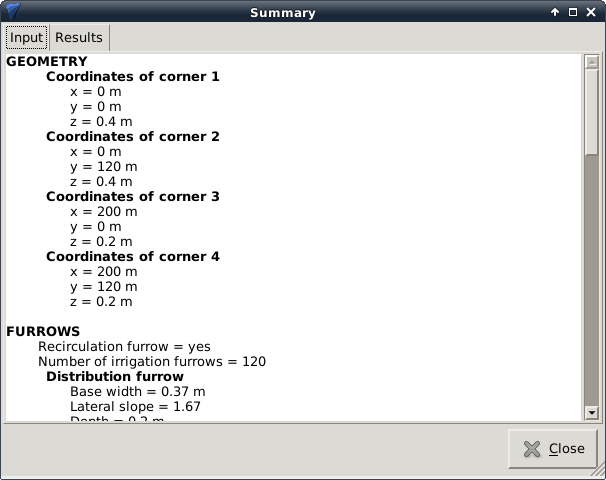
\includegraphics[width=0.45\textwidth]{images/sumarioEN.png}
\qquad
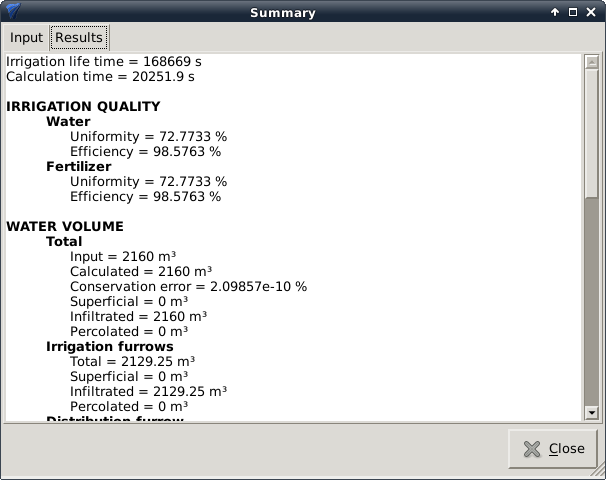
\includegraphics[width=0.45\textwidth]{images/sumario2EN.png}
\caption{Summary of the input data (Left) and results (Right)}\label{wInforme}
\end{center}
\end{figure}


%%%%%%%%%%%%%%%%%%%%%%%%%%%%%%%%%%%%%%%%%%%%%%%%%%%%%%%%%%%%%%%%%%%%%%%%%%%%%%%%%%%%%%%%%%%%%%%%%%%%%%%%5

\cleardoublepage

\chapter{Input and Output files format}

In program \emph{Surcos}, the input and output files are stored in a single common folder whose name
can be chosen by the user. However, the input and output files are plain ASCII files with a fixed name
that follows the structure detailed in next sections


\section{Input files}

\subsection{The geometry file: field.in}

The geometry file is always named:
\begin{itemize}
\item Case\_folder$\backslash$field.in
\end{itemize}

This file contains the following set of numbers:\\
$o$ $n$ $s$\\
$x_1$ $y_1$ $z_1$\\
$x_2$ $y_2$ $z_2$\\
$x_3$ $y_3$ $z_3$\\
$x_4$ $y_4$ $z_4$\\
$b_b$ $z_b$ $H_b$ $D_b$ $R_b$ $\epsilon_b$ $r_b$ $K_b$ $a_b$ $i_b$ $d_b$
	$h_b$ $Q_b$ $c_b$\\
$b_i$ $z_i$ $H_i$ $D_i$ $R_i$ $\epsilon_i$ $r_i$ $K_i$ $a_i$ $i_i$ $d_i$
	$h_i$ $Q_i$ $c_i$\\
$b_c$ $z_c$ $H_c$ $D_c$ $R_c$ $\epsilon_c$ $r_c$ $K_c$ $a_c$ $i_c$ $d_c$
	$h_c$ $Q_c$ $c_c$\\
with:
\begin{description}
\item[$o$] 1 if there is recirculation furrow, 0 otherwise.
\item[$n$] Number of irrigation furrows. 0 if there is a single furrow. 
           In that case, the flow in the distribution furrow is simulated.
\item[$s$] Fertilizer solubility.
\item[$x_j$, $y_j$, $z_j$] Spatial coordinates of vertex $j$ defining one corner of the 
	furrow network plot.  
\item[$b_k$] Base width in furrow $k$.
\item[$z_k$] Lateral slope in furrow $k$.
\item[$H_k$] Maximum depth in furrow $k$.
\item[$D_k$] Furrow separation at furrow $k$.
\item[$R_k$] Water retention capacity in furrow $k$.
\item[$\epsilon_k$] Burguete aerodynamic roughness coefficient ($\epsilon>0$) or Gauckler-Manning 
            roughness coefficient($\epsilon=0$) at furrow $k$.
\item[$r_k$] Gauckler-Manning number ($\epsilon=0$) or Burguete roughness characteristic length
            ($\epsilon>0$) at furrow $k$.
\item[$K_k$] Kostiakov infiltration coefficient at furrow $k$.
\item[$a_k$] Kostiakov infiltration power at furrow $k$.
\item[$i_k$] Infiltration saturated rate at furrow $k$.
\item[$d_k$] Diffusion coefficient at furrow $k$.
\item[$h_k$] Initial surface water depth at furrow $k$.
\item[$Q_k$] Initial surface water discharge at furrow $k$.
\item[$c_k$] Initial fertilizer concentration at furrow $k$.
\end{description}
The subindex label $k$ represents: $b$ for the distribution furrow, $i$ for all the irrigation furrows 
(they are all assumed to share the same geometry properties) and $c$ for the recirculation furrow.

\subsection{Inlet water and fertilizer file: input.in}

Water and fertilizer inlet is defined in a file named:
\begin{itemize}
\item Case\_folder$\backslash$input.in
\end{itemize}

The following set of data must be provided:\\
$n_w$ $n_s$\\
$x_1$ $y_1$ $I_1$ $F_1$ $q_1$\\
$\cdots$\\
$x_{n_w}$ $y_{n_w}$ $I_{n_w}$ $F_{n_w}$ $q_{n_w}$\\
$x_1$ $y_1$ $I_1$ $F_1$ $q_1$\\
$\cdots$\\
$x_{n_s}$ $y_{n_s}$ $I_{n_s}$ $F_{n_s}$ $q_{n_s}$\\
with:
\begin{description}
\item[$n_w$, $n_s$] the number of water and fertilizer inlet points respectively,
\item[$x_i$] $x$ coordinate of the $i$ inlet point,
\item[$y_i$] $y$ coordinate of the $i$ inlet point,
\item[$I_i$] initial time at the $i$ inlet point,
\item[$F_i$] final time at the $i$ inlet point,
\item[$q_i$] Inlet discharge at the $i$ inlet point, in $m^3/s$ if it is a water inlet or in 
	 $kg/s$ when it is a fertilizer inlet.
\end{description}
Note that first the $n_w$ water inlet points must be defined and then the $n_s$ fertilizer inlet points.

\subsection{Simulation time file: times.in\label{SecTiempos}}

The relevant time data in the simulation are defined in file:
\begin{itemize}
\item Case\_folder$\backslash$times.in
\end{itemize}

This file contains the following information:\\
$t_f$ $cfl$ $t_m$\\
where:
\begin{description}
\item[$t_f$] is the total simulation time,
\item[$cfl$] is the CFL number controlling the time step,
\item[$t_m$] is the time interval to write intermediate numerical results in a file.
\end{description}

\subsection{Grid file: mesh.in}

The number of grid computational grid cells is defined in file:
\begin{itemize}
\item Case\_folder$\backslash$mesh.in
\end{itemize}

This file contains:\\
$n_d$ $n_i$\\
with:
\begin{description}
\item[$n_d$] number of cells inserted in the distribution/recirculation furrows between each pair of irrigation furrows,
\item[$n_i$] number of cells in every irrigation furrow.
\end{description}

\subsection{Probes file: probe.in}

The measurement points or probes are specified in the file:
\begin{itemize}
\item Case\_folder$\backslash$probe.in
\end{itemize}

This file contains the following data:\\
$n_p$\\
$x_1$ $y_1$\\
$\cdots$\\
$x_{n_p}$ $y_{n_p}$\\
with:
\begin{description}
\item[$n_p$] total number of probes,
\item[$x_i$] $x$ coordinate of the location of the $i$ probe,
\item[$y_i$] $y$ coordinate of the location of the $i$ probe.
\end{description}

\subsection{Model file: model.in}

The models used are defined in the file:
\begin{itemize}
\item Case\_folder$\backslash$model.in
\end{itemize}

This file contains the following data:\\
$m_f$ $m_i$ $m_u$ $m_a$\\
with:
\begin{description}
\item[$m_f$] 1 if there is fertilizer transport, 0 otherwise.
\item[$m_i$] 1 if there is infiltration, 0 otherwise.
\item[$m_u$] 1 if there is turbulent diffusion, 0 otherwise.
\item[$m_a$] 1 if the Boussinesq convection model is used, 0 if the simple model is used.
\end{description}

\section{Results files}

In program \emph{Surcos} the results are gathered in files according to the following names: 
\begin{description}
\item[00b] Distribution furrow.
\item[00c] Recirculation furrow.
\item[xxx] Irrigation furrow, with $xxx$ representing the furrow number with 3
	digits. The furrow numbering goes from 0 to $n$-1 with $n$ the total number of irrigation furrows.
\end{description}

The results files are written in the same folder where the input data files are. The program generates
3 different results files, all of them in ASCII format.

\subsection{Longitudinal profile files (xxx-yyy.out)}

\emph{Surcos} generates a file to store the longitudinal profile of every variable in every furrow for every
intermediate time as defined in section~\ref{SecTiempos}). The name of these files is as follows:

\begin{itemize}
\item $xxx-yyy.out$
\end{itemize}
where $xxx$ represents the furrows name with the above described codification and $yyy$ represents
the intermediate time step with 3 digits.

The profiles are provided using files with 12 columns in the form:\\
\begin{tabular}{cccccccccccc}
$x_1$& $h_1$& $A_1$& $Q_1$& ${z_s}_1$& ${z_f}_1$& $-{A_i}_1$& $c_1$&
	$-{A_{ci}}_1$& $-{A_p}_1$& $-{A_{cp}}_1$& $\beta_1$\\
&&&&&&$\cdots$\\
$x_n$& $h_n$& $A_n$& $Q_n$& ${z_s}_n$& ${z_f}_n$& $-{A_i}_n$& $c_n$&
	$-{A_{ci}}_n$& $-{A_p}_n$& $-{A_{cp}}_n$& $\beta_n$
\end{tabular}\\\\
with:
\begin{description}
\item[$x_i$] the longitudinal coordinate of the $i$ grid point,
\item[$h_i$] the surface water depth of the $i$ grid point,
\item[$A_i$] the surface wetted cross section of the $i$ grid point,
\item[$Q_i$] the surface water discharge of the $i$ grid point,
\item[${z_s}_i$] the water surface elevation of the $i$ grid point,
\item[${z_f}_i$] the bed level elevation of the $i$ grid point,
\item[$-{A_i}_i$] the infiltrated water volume (negative) per unit furroe length of the $i$ grid point,
\item[$c_i$] the surface fertilizer concentration of the $i$ grid point,
\item[$-{A_{ci}}_i$] the mass of fertilizer infiltrated (negative) per unit furrow length of the $i$ grid point,
\item[$-{A_p}_i$] the volume of percolated water per unit furrow length of the $i$ grid point,
\item[$-{A_{cp}}_i$] the mass of percolated fertilizer per unit furrow length of the $i$ grid point,
\item[$\beta_i$] the Boussinesq convection coefficient of the $i$ grid point, 
\item[$n$] the number of grid points in the furrow.
\end{description}

\subsection{Advance and recession times files (xxx.out)}

\emph{Surcos} generates files with information concerning the advance and recession times in every furrow. 
The names of the files are in the following form: 
\begin{itemize}
\item $xxx.out$
\end{itemize}
where $xxx$ represents the name of the furrow with the above described codification. 

These files contain 3 columns in the form:\\
\begin{tabular}{ccc}
$x_1$& ${t_a}_1$& ${t_r}_1$\\
&$\cdots$\\
$x_n$& ${t_a}_n$& ${t_r}_n$\\
\end{tabular}\\\\
with:
\begin{description}
\item[$x_i$] the longitudinual aoordinate of the $i$ grid cell,
\item[${t_a}_i$] the advance time for the $i$ grid cell,
\item[${t_r}_i$] the recession time for the $i$ grid cell,
\item[$n$] the number of grid points in the furrow.
\end{description}

\subsection{Probe files (probes.out)}

The files where the probe information is stored are called \emph{probes.out}. This file is written with the following format:\\
\begin{tabular}{cccccc}
$t_0$ & $h_{1,0}$ & $c_{1,0}$ & $\cdots$ & $h_{n_p,0}$ & $c_{n_p,0}$\\
&&&$\vdots$\\
$t_{n_t}$ & $h_{1,n_t}$ & $c_{1,n_t}$ & $\cdots$ & $h_{n_p,n_t}$ & $c_{n_p,n_t}$
\end{tabular}\\\\
with:
\begin{description}
\item[$t_j$] the $j$ time level, with 0 the initial time,
\item[$h_{i,j}$] the surface water depth measured in probe $i$ at time $j$,
\item[$c_{i,j}$] the surface fertilizer concentration measured in probe $i$ at time $j$,
\item[$n_p$] the total number of probes,
\item[$n_t$] the total number of time steps.
\end{description}

%\cleardoublepage

%\bibliography{bib/references}
%\cleardoublepage

\end{document}
